\chapter{Resultados e discussão}
\label{cap:resultados}

\section{Comparação principal no Gallagher}
A Tabela~\ref{tab:principal} reúne os resultados da execução congelada de 28 de setembro de 2026. As cinco configurações usam as mesmas 20 consultas e a mesma galeria de 588 candidatos por consulta. Portanto, a comparação entre linhas mantém constantes consultas, relevância e exclusão da fotografia de origem. Os valores são apresentados com seis casas decimais para permitir confronto com os arquivos de origem; essa precisão de apresentação não representa precisão estatística.

\begin{table}[htbp]
\centering\caption{Recuperação no Gallagher: métricas médias por consulta.}\label{tab:principal}
\resizebox{\textwidth}{!}{\begin{tabular}{lrrrrr}
\toprule
Método & P@5 & P@10 & R@5 & R@10 & mAP \\
\midrule
Somente face & 0,900000 & 0,680000 & 0,577119 & 0,687856 & 0,952261 \\
Somente global & 0,260000 & 0,195000 & 0,203512 & 0,234712 & 0,280864 \\
Fusão 0,9/0,1 & 0,900000 & 0,680000 & 0,577119 & 0,687856 & 0,946274 \\
Fusão 0,7/0,3 & 0,840000 & 0,675000 & 0,540571 & 0,682856 & 0,901460 \\
Fusão 0,5/0,5 & 0,770000 & 0,630000 & 0,481033 & 0,634905 & 0,813297 \\
\bottomrule
\end{tabular}
}
\fonte{elaboração a partir de \texttt{fusion\_metrics.csv}, execução atual.}
\end{table}

O componente facial isolado obteve mAP de 0,952261, enquanto o componente global isolado atingiu 0,280864. A fusão com peso facial de 0,9 obteve 0,946274, seguida das configurações 0,7 e 0,5, com 0,901460 e 0,813297. Assim, nenhum dos três pesos de fusão superou a configuração facial na média de AP. A Figura~\ref{fig:map} facilita a comparação das magnitudes, mas não acrescenta observações às mesmas 20 consultas.

\begin{figure}[htbp]
\centering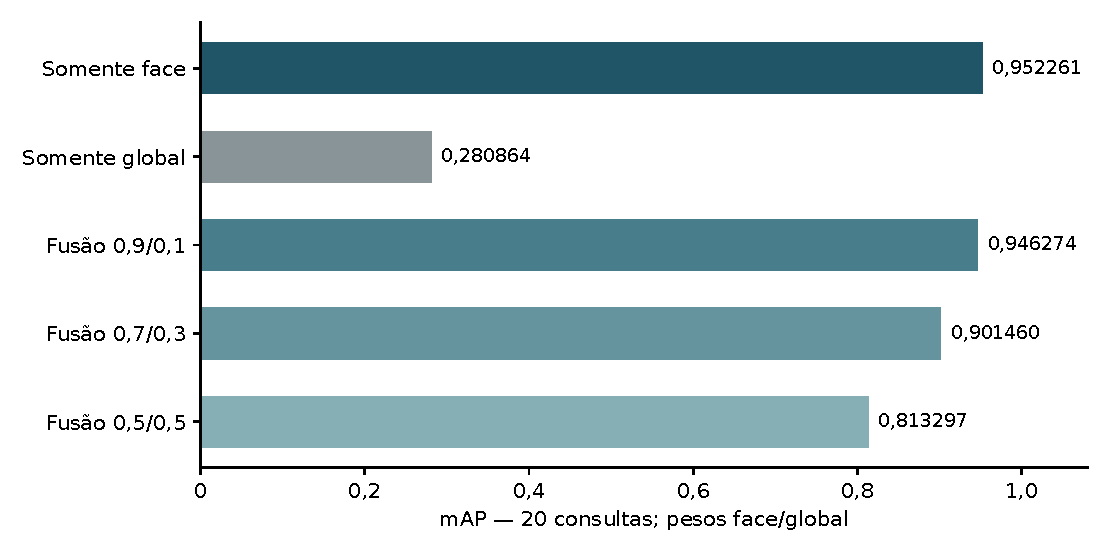
\includegraphics[width=\textwidth]{figuras/map_gallagher.pdf}
\caption{mAP das configurações avaliadas no Gallagher.}\label{fig:map}
\fonte{elaboração a partir das métricas agregadas da execução atual.}
\end{figure}

A diferença entre a fusão 0,9/0,1 e a face isolada foi de aproximadamente $-0,005987$ em mAP, ou $-0,599$ ponto percentual quando a medida é expressa em porcentagem. Essa diferença é pequena em comparação com as demais configurações, mas seu sinal não sustenta uma alegação de ganho agregado. Com pesos faciais de 0,7 e 0,5, as diferenças foram de aproximadamente $-0,050801$ e $-0,138964$. A ordenação das médias é compatível com a perda de adequação do escore global à relevância por identidade neste protocolo. Não demonstra, por si só, que o fundo causou cada erro.

Os valores de P@5, P@10, R@5 e R@10 são idênticos, nas casas apresentadas, entre face isolada e fusão 0,9/0,1. Isso não implica rankings iguais. As métricas em cortes dependem da quantidade de relevantes recuperados até cada posição, enquanto AP considera também sua distribuição ao longo do ranking completo. Trocas de ordem dentro de um corte e alterações depois do décimo resultado podem modificar AP sem alterar aquelas quatro medidas. Além disso, são médias: valores agregados iguais podem ocultar diferenças entre consultas.

A precisão média de 0,9 nos cinco primeiros resultados indica que esse conjunto inicial foi predominantemente relevante para as consultas selecionadas. O recall médio de aproximadamente 0,577 nesse corte mostra que esse mesmo resultado não equivale à recuperação de todas as fotografias relevantes. Pessoas com muitas fotografias têm denominadores maiores de recall. Por isso, a precisão no topo e a cobertura da coleção respondem a perguntas distintas e devem acompanhar a interpretação de mAP.

\section{Análise pareada por consulta}
Para examinar a heterogeneidade ocultada pelas médias, calculou-se, para cada consulta $q$, $\Delta\mathrm{AP}(q)=\mathrm{AP}_{\text{método}}(q)-\mathrm{AP}_{\mathrm{face}}(q)$. A análise usa os resultados já gravados, sem executar novamente o extrator ou o avaliador. Empates são contados com tolerância numérica de $10^{-12}$.

\begin{table}[htbp]
\centering\caption{Diferenças pareadas de AP em relação ao componente facial.}\label{tab:pareados}
\resizebox{\textwidth}{!}{\begin{tabular}{lrrrrr}
\toprule
Método contra face & Ganhos & Empates & Perdas & Média $\Delta$AP & Mediana \\
\midrule
Somente global & 0 & 1 & 19 & -0,671397 & -0,762430 \\
Fusão 0,9/0,1 & 2 & 9 & 9 & -0,005987 & 0,000000 \\
Fusão 0,7/0,3 & 1 & 7 & 12 & -0,050801 & -0,017696 \\
Fusão 0,5/0,5 & 0 & 4 & 16 & -0,138964 & -0,091663 \\
\bottomrule
\end{tabular}
}
\fonte{cálculo documental sobre as 100 linhas de \texttt{fusion\_metrics\_per\_query.csv}.}
\end{table}

A fusão 0,9/0,1 melhora duas consultas, empata nove e piora nove. Seu maior ganho é de 0,05 e a maior perda é de 0,0625 em AP. Portanto, existem benefícios pontuais, mas eles não compensam as perdas na média. Na configuração 0,7/0,3, uma consulta melhora, sete empatam e doze pioram; a maior perda chega a 0,35. Na configuração 0,5/0,5, não há ganho, quatro consultas empatam e dezesseis pioram; a maior perda é aproximadamente 0,776474. O componente global isolado apresenta um empate e dezenove perdas, sem ganho, em relação ao facial.

\begin{figure}[htbp]
\centering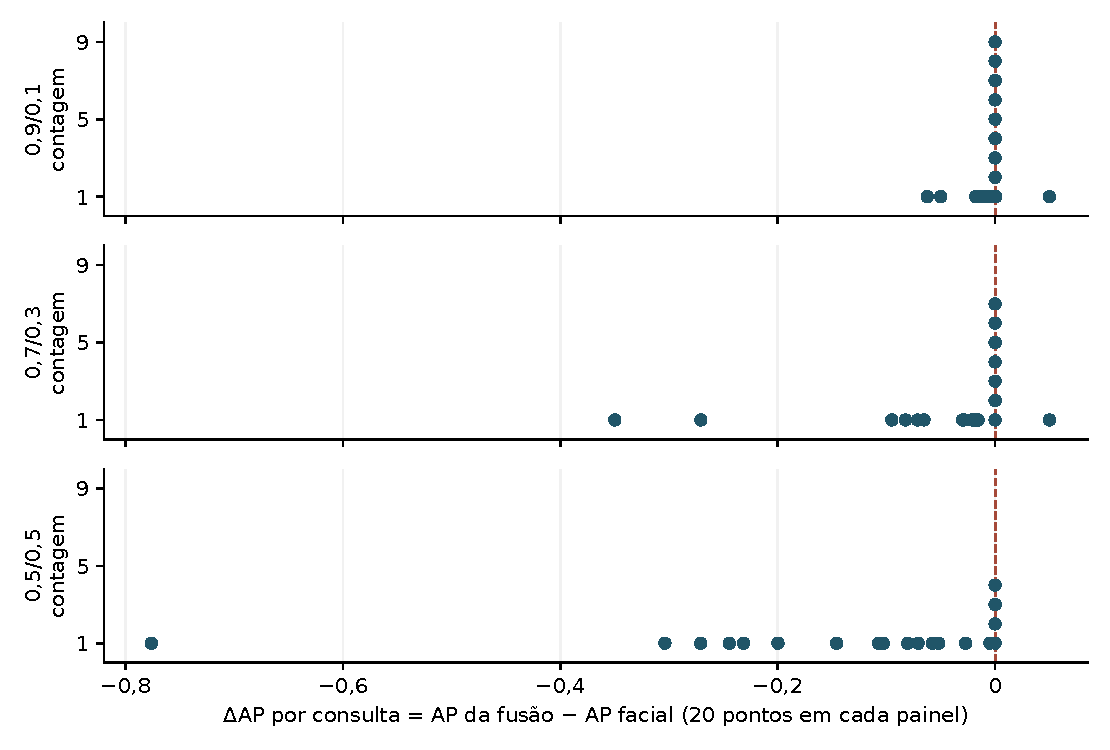
\includegraphics[width=\textwidth]{figuras/deltas_pareados.pdf}
\caption{Distribuição das diferenças de AP das fusões. Cada painel contém 20 observações; pontos de mesmo valor são empilhados.}\label{fig:deltas}
\fonte{elaboração sobre métricas por consulta, sem exibir identificadores.}
\end{figure}

Na Figura~\ref{fig:deltas}, a linha vertical marca ausência de diferença. O aumento da dispersão à esquerda, quando cresce a participação do escore global, torna visível um efeito que uma única média resumiria de forma incompleta. A mediana da fusão 0,9/0,1 é zero, mas sua média é negativa; assim, não se deve substituir uma medida pela outra conforme a narrativa desejada. Ambas indicam aspectos complementares da distribuição observada.

As observações não constituem vinte repetições independentes de um experimento aleatório. Há dependência entre fotografias, pessoas e contextos compartilhados, e duas consultas podem ter origem na mesma imagem. Também houve seleção por frequência e por sucesso na preparação da consulta. Não foram calculados valores de significância, intervalos de confiança populacionais ou efeitos causais. A contagem de ganhos e perdas é descritiva e se restringe às consultas congeladas.

\section{Resultados auxiliares}
\begin{table}[htbp]
\centering\caption{Resultados auxiliares em protocolos locais distintos.}\label{tab:auxiliares}
\begin{tabular}{lrrrl}\toprule
Base & Consultas & Candidatos & mAP & Componente\\\midrule
LFW & 1.672 & 13.184 & 0,965136 & Facial\\
Holidays & 500 & 1.490 & 0,842612 & Global\\\bottomrule
\end{tabular}
\fonte{\texttt{face\_metrics.csv} e \texttt{global\_metrics.csv} da execução atual.}
\end{table}

O resultado em LFW mostra que o fluxo facial foi aplicado a uma coleção maior sob o protocolo local de recuperação. Não é acurácia oficial de verificação por pares. As consultas e a galeria são condicionadas às fotografias indexadas: 48 das 13.233 imagens examinadas não tiveram detecção e não integram as 13.185 imagens indexadas. A seleção do maior rosto na consulta difere do procedimento orientado por anotação usado no Gallagher. Essas escolhas impedem usar 0,965136 como medida geral de reconhecimento facial ou como comparação direta com resultados publicados no protocolo oficial de LFW.

O resultado em Holidays indica que o descritor global e o ranking produzem uma recuperação mensurável quando a relevância corresponde aos grupos visuais daquela coleção. Não prova que esse escore seja apropriado para localizar uma identidade. Também não permite comparar numericamente seu mAP com o de Gallagher: mudam a tarefa, as consultas, a galeria e a definição de relevância. A implementação local de AP difere da integração trapezoidal do avaliador oficial de Holidays, e foram identificados três pares de arquivos idênticos em grupos diferentes. Esses limites são preservados na interpretação, sem corrigir retrospectivamente a execução congelada.

\section{O que a literatura permite interpretar}
Os trabalhos sobre reconhecimento de pessoas em álbuns exploram pistas de diferentes regiões e relações contextuais \cite{Zhang2015,Oh2015,Li2016}. Sua motivação ajuda a compreender por que informação além da face pode ser útil em certas condições. Entretanto, usar redes treinadas para regiões específicas ou inferência contextual estruturada não equivale a combinar linearmente uma similaridade facial com um descritor global de classificação. Os resultados desta monografia avaliam essa combinação específica, e não toda a classe de métodos contextuais.

Há pelo menos três explicações plausíveis para a ausência de ganho médio. Primeiro, a identidade facial e a aparência global respondem a relações diferentes entre fotografias. Segundo, a transformação afim dos cossenos estabelece uma faixa comum, mas não calibra as distribuições de escores. Terceiro, o desempenho facial elevado nas consultas aceitas deixa pouco espaço para ganho e ainda permite perdas por reordenação. Essas explicações são hipóteses de interpretação. O estudo não realizou ablações suficientes para separá-las ou quantificar a contribuição causal de cada uma.

Também não se avaliou se outro descritor global, outro conjunto de pesos, uma regra adaptativa ou uma estratégia treinada com conjunto de validação independente produziria resultado diferente. Escolher pesos depois de observar as consultas de teste não forneceria uma validação independente. Assim, o resultado negativo para as fusões fixas é informativo sem justificar a conclusão de que contexto visual nunca ajuda.

\section{Validação de engenharia e limites de uso}
O fechamento técnico registra 93 testes aprovados e uma aceitação operacional com 171 fotografias, das quais 59 HEIC e 112 JPEG, e 552 representações faciais. Esses números são evidências registradas anteriormente; os testes não foram repetidos durante a redação. A aceitação verificou operações concretas no acervo privado e preservação dos originais. Não constituiu estudo de usabilidade com participantes, validação de consentimento para divulgação ou avaliação quantitativa independente de recuperação.

O registro de 189 segundos distribuídos por 12 pontos de verificação não é um ensaio de latência. Não houve controle suficiente de aquecimento, cache, repetição ou carga para transformá-lo em benchmark. Da mesma forma, o uso de GPU e a busca vetorizada não demonstram escalabilidade em milhões de imagens. A implementação não ativa FAISS, e essa parte da proposta inicial permanece fora do escopo realizado.

As limitações abrangem validade interna, externa e de construção. A preparação condiciona quais consultas chegam à avaliação; o extrator pode ter exposição prévia a identidades das bases, sem garantia de separação de treinamento; as fotografias e consultas são dependentes; e o resultado de recuperação não equivale a satisfação do usuário. Além disso, persistem limites de auditoria: os arquivos conservam métricas por consulta e os dez primeiros resultados, mas não todos os rankings completos necessários para recalcular AP independentemente sem nova execução. O pacote documental permite conferir médias, diferenças e procedência, sem alegar reprodução integral a partir apenas desse pacote.

